

\documentclass[14pt]{beamer}
\usepackage{pgf,tikz,pgfpages,amsmath,bm,fancyvrb,animate}
\usepackage{graphicx,bera,booktabs}
\usepackage[australian]{babel}
\usepackage[utf8]{inputenc}

\usetheme{Monash}
\def\biz{\begin{itemize}[<+-| alert@+>]}
\def\eiz{\end{itemize}}
\def\ben{\begin{enumerate}[<+-| alert@+>]}
\def\een{\end{enumerate}}

\graphicspath{{../figures/}{../figures/book_figures/Chapter6/}}

\title[5. Other dimensionality reduction methods]{Business Analytics}
\author{Week 5\\ Other dimensionality reduction methods}


\DefineShortVerb{\"}
\def\FancyVerbFormatCom{\color[rgb]{0.6,0,1}\relax}


\begin{document}

\begin{frame}[plain]{}
\maketitle
\begin{textblock}{11}(0.5,1.3){\color{white}\large
\textbf{ETC3250}}
\end{textblock}
\end{frame}


\begin{frame}{Dimensionality reduction}\large

\begin{itemize}
\item Wy dimensionality reduction?
\begin{itemize}
	\item Curse of dimensionality
	\item Intrinsic dimensionality
	\item Visualization
\end{itemize}

\item Dimensionality reduction methods
\begin{itemize}
\item Feature selection vs feature extraction (examples? advantages?)
\item Unsupervised vs supervised
\item Linear vs nonlinear
\end{itemize}

\item Principal components analysis (PCA)
\begin{itemize}
\item PCA produces a low-dimensional representation of a dataset. It finds a sequence of linear combinations of the variables that have maximal variance, and are mutually uncorrelated.
\item PCA is linear and unsupervised feature extraction method
%\item Variants of PCA: Nonlinear PCA, Kernel PCA, Sparse PCA, etc.
\end{itemize}

\end{itemize}


\end{frame}

%%%%%%%%%% PLS %%%%%%%%%%
\begin{frame}{\normalsize Dimensionality reduction in regression}


\begin{itemize}
	\item How would you reduce dimensionality in linear regression?
	\item How would use PCA to reduce dimensionality in linear regression?
	\item Principal components regression (PCR): use PCA to construct the first $M$ principal components, $Z_1$, \dots, $Z_M$, and then fit a linear regression model using these components.
	\item Assumption: \emph{the directions in which $X_1$, \dots, $X_p$ show the most variation are the directions that are associated with $Y$}. When is PCR better than traditional least squares?
\end{itemize}

\end{frame}

\begin{frame}{Partial least squares}

\begin{itemize}
\item With PCR, the components are identified in an \textbf{unsupervised way}. No guarantee that the directions that \textcolor{blue}{best explain the predictors} will also be the \textcolor{blue}{best directions to use for predicting the response $Y$}. How would you use the response $Y$ to reduce dimensionality?
\pause
\item Partial least squares (PLS) is a \textbf{supervised} alternative to PCR. Same procedure as PCR, but the new features are identified in a supervised way. Roughly speaking, PLS attempts to find directions that help \textcolor{blue}{explain both the response and the predictors}.
%PLS seeks directions that have high variance and have high correlation with the response

\end{itemize}

\end{frame}

\begin{frame}{Partial least squares}\small

\begin{enumerate}
	\item Standardize the $p$ predictors
	\item Compute the first direction $Z_1$ by setting each $\phi_{j1}$ in $Z_1 = \sum_{j = 1}^p \phi_{j1} X_j$ equal to the coefficient from the simple linear regression of $Y$ onto $X_j$ (see Figure)
	\item For the second direction $Z_2$, we first adjust each of the variables for $Z_1$, by regressing each variable on $Z_1$, and taking residuals, say $X'_j$. These residuals represent the remaining information that has not been explained by the the first PLS direction $Z_1$. We then compute $Z_2$ using $X'_j$ as $Z_1$ was computed from $X_j$
	\item We can compute $Z_1, \dots, Z_M$ iteratively. Then we use least squares to fit a linear model using $Z_1, \dots, Z_M$ as for PCR. How to choose $M$?
\end{enumerate}

\end{frame}

\begin{frame}{PLS Example}

\fullwidth{6-21}

\begin{textblock}{12}(0.6,8.8)
\textcolor[RGB]{0,159,134}{Solid line: first PLS direction.}\qquad 
\textcolor[RGB]{0,159,134}{Dotted line: first PC.}
\end{textblock}
\end{frame}


\begin{frame}{Partial least squares}

\begin{itemize}
\item There are two variants of PLS: PLS1 (one response variable) and PLS2 (at least two response variables).
\item In practice, PLS1 is not better than ridge regression or PCR (PLS reduces bias but can potentially increase variance).
\item PLS2 is a useful tool for multiresponse regression.
\item Other supervised dimensionality reduction methods: CCA, LDA, etc.
\end{itemize}

\end{frame}



%%%%%%%%%%%% Nonlinear dimension reduction methods  %%%%%%%%%%%%

\begin{frame}{Computation of PCs}

\begin{itemize}

\item Singular value decomposition

\begin{itemize}
\item $\bm{X} = \bm{U}\bm{\Lambda}\bm{V}'$ with $\bm{U}'\bm{U}=\bm{I}$ and $\bm{V}'\bm{V}=\bm{I}$
\item $\bm{\Phi} = \bm{V} \rightarrow \bm{Z} = \bm{X}\bm{\Phi}$
\end{itemize}
	
\item Eigenvalue decomposition

\begin{itemize}
\item $\bm{C} = \bm{X'X}$ where the columns of $\bm{X}$ are scaled
\item $\bm{C}=\bm{V}\bm{D}\bm{V}'$ with $\bm{V}'\bm{V}=\bm{I}$
\item $\bm{\Phi} = \bm{V} \rightarrow \bm{Z} = \bm{X}\bm{\Phi}$
\end{itemize}

\end{itemize}

%\vspace{.5cm}
%\centerline{\textcolor{blue}{PCA from distances only?}}

\end{frame}

\begin{frame}{Computation of PCs}

Suppose that instead of measuring a $n \times p$ dataset $\bm{X} = [x_{ij}]$, we were only given a pairwise distance matrix $\Delta$ where

$$ \Delta_{ij} = \lVert x_i - x_j \rVert_2, \quad i, j = 1, \dots, N$$
i.e. we do not know  the points themselves. Can we recover the principal components, or equivalently the lower-dimension representation $\bm{Z}$?

\end{frame}


\begin{frame}{\normalsize Classical multidimensional scaling}

\begin{itemize}
	\item The answer is: yes, with classical multidimensional scaling
		\begin{itemize}
		\item First recover the inner product $\bm{XX'}$ from $\Delta$
		\item Then, use eigendecomposition to recover $\bm{Z}$
		\end{itemize}
	\item Classical MDS finds a lower-dimensional representation $z_1, \dots, z_n \in R^k$, for $k << p$ such that $\lVert z_i - z_j \rVert_2 \approx \Delta_{ij}$, for every $i, j = 1, \dots, N$.
	\item If $\Delta_{ij}$ are euclidean distances between the rows of $\bm{X}$, then MDS is equivalent to PCA (see code).
\end{itemize}

\end{frame}


\begin{frame}{Multidimensional scaling}

\begin{itemize}
\item Multidimensional scaling can be applied to any $\Delta_{ij}$, not just Euclidean distances
\item In this case, we don't compute principal component scores, and the lower-dimensional representation can be a nonlinear function of the data 
\item When do we need to use non-Euclidean distances?
\end{itemize}

\centerline{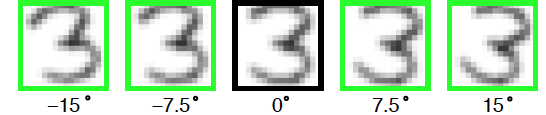
\includegraphics[width=.6\textwidth]{digits}}
We wish to remove the effect of rotation in measuring distances between two digits

% other distances

% objective function of MDS

% stree functions?

% Isomap (with graphs)

% Nonlinear dimensionality reduction 
\end{frame}

\begin{frame}{Isometric feature mapping}



\includegraphics[width=\textwidth]{isomap}

{\small (From Tenenbaum et al. (2000), ``A global geometric framework for nonlinear dimensionality reduction'')}

\begin{itemize}
\item Construct a graph $G = (V, E)$ based on the structure between $x_1, \dots, x_n$.
\item Then, define a graph distance $\Delta_{ij}^{\text{Isomap}}$ between $i$ and $j$, and use MDS for the low-dimensional representation
\end{itemize}



\end{frame}





\begin{frame}{\large Dimensionality reduction methods}

\begin{itemize}
\item Feature selection vs feature extraction
\item Linear and nonlinear
\item Unsupervised and supervised
\item Low-dimensional representation with maximum variance, that retains local properties of the data, etc.
\item \textbf{Linear PCA}, Nonlinear PCA, Kernel PCA, Sparse PCA, etc.
\item \textbf{MDS}, ICA, LDA, etc.
\item \textbf{PLS}, CCA, FA, etc.
\item \textbf{Isomap}, diffusion maps, MVU, LLE, t-SNE, autoencoders, etc.
\end{itemize}
 

\end{frame}




\end{document}